\documentclass{standalone}

\usepackage{tikz}
\usepackage{pgfplots}
\begin{document}
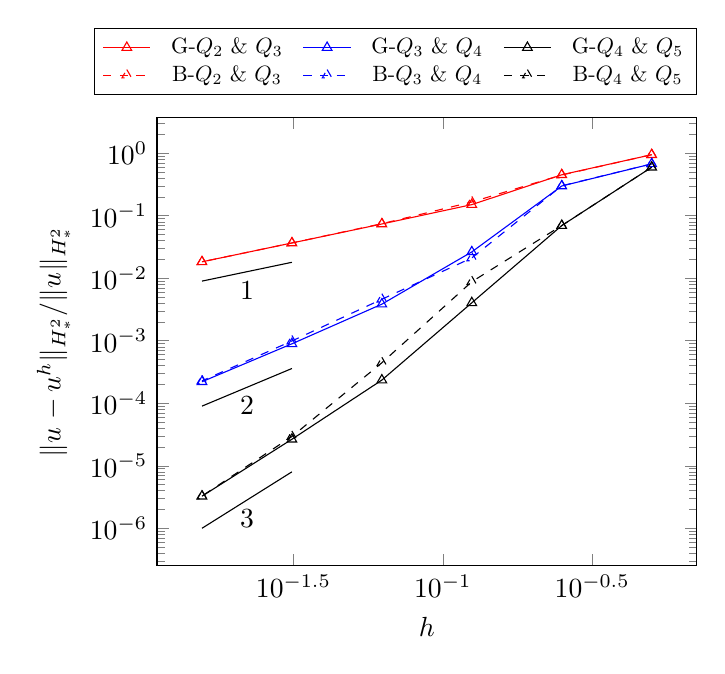
\begin{tikzpicture}
    \begin{loglogaxis}[
        legend columns=3,
    	legend style={at={(1,1.2)}, nodes={scale=0.8, transform shape}, column sep=.2cm},
        xlabel=$h$,
        ylabel=${\|u_{}-u^{h}\|_{H^2_*}}/{\|u_{}\|_{H^2_*}}$ 
    ]


    \addplot [color=red,mark=triangle] plot coordinates {

        (.5,    0.947573)
        (.25,   0.452374)
        (.125,  0.150636)
        (.0625,   0.0738313)
        (0.03125,   0.0366665 )
        (0.015625,  0.0183142 )
    };

    \addplot [color=blue,mark=triangle] plot coordinates {

        (.5,    0.675618)
        (.25,   0.29897)
        (.125,      0.0263881)
        (.0625,     0.00385068)
        (0.03125,   0.000894183)
        (0.015625,  0.000221005)
    };

    \addplot [color=black,mark=triangle] plot coordinates {

        (.5,    0.597089)
        (.25,   0.069544)
        (.125,      0.00404805)
        (.0625,     0.00023493)
        (0.03125,   2.65706e-05)
        (0.015625,  3.25804e-06)
    };

    
    \addplot [color=red,mark=triangle, dashed] plot coordinates {

        (.5,    0.947573)
        (.25,   0.448626)
        (.125,      0.165961)
        (.0625,     0.0745943)
        (0.03125,   0.0366899)
        (0.015625,  0.0183149)
    };

    \addplot [color=blue,mark=triangle, dashed] plot coordinates {

        (.5,    0.675618)
        (.25,   0.300972)
        (.125,      0.0211338)
        (.0625,     0.0046142 )
        (0.03125,   0.000991629)
        (0.015625,  0.0002282)
    };

    \addplot [color=black,mark=triangle, dashed] plot coordinates {

        (.5,    0.597089)
        (.25,   0.0697155)
        (.125,      0.00879059)
        (.0625,     0.000444331)
        (0.03125,   2.93938e-05)
        (0.015625,  3.28279e-06)
    };


    \addplot [black] plot coordinates {

        (0.03125,    0.0180)
        (0.015625,   .009)
    } node[pos=0.5,anchor=north]{$1$};

    \addplot [black] plot coordinates {

        (0.03125,    3.6000e-04)
        (0.015625,   0.00009)
    } node[pos=0.5,anchor=north]{$2$};

    \addplot [black] plot coordinates {

        (0.03125,    8.0000e-06)
        (0.015625,   1e-6)
    } node[pos=0.5,anchor=north]{$3$};

    \legend{G-$Q_2$ $\&$ $Q_3$\\G-$Q_3$ $\&$ $Q_4$\\G-$Q_4$ $\&$ $Q_5$\\B-$Q_2$ $\&$ $Q_3$\\B-$Q_3$ $\&$ $Q_4$\\B-$Q_4$ $\&$ $Q_5$\\}
    \end{loglogaxis}
\end{tikzpicture}

\end{document}



% 1.02271   0.947573
% 0.393272   0.452374
% 0.0360061   0.150636
% 0.00802147   0.0738313
% 0.00193664   0.0366665
% 0.00048126   0.0183142

% 0.694232   0.675618
% 0.166681   0.29897
% 0.0040645   0.0263881
% 6.81819e-05   0.00385068
% 1.6304e-06   0.000894183
% 7.29714e-08   0.000221005

% 0.351814   0.597089
% 0.0178482   0.069544
% 0.000449695   0.00404805
% 2.92727e-06   0.00023493
% 3.81391e-08   2.65706e-05
% 7.7457e-10   3.25804e-06